% Narrative candidate; the approved main_v10_final4.tex and PDF remain frozen.
\documentclass[conference]{IEEEtran}
\usepackage{cite}
\usepackage{amsmath,amssymb}
\usepackage{graphicx,booktabs,placeins,url}
\newif\iffourfigures\fourfigurestrue
\begin{document}
\title{From Connection Loss to Collision: Closed-Loop Fault Assessment of a Fly-Connectome SNN}
\author{\IEEEauthorblockN{Shuchao Gao}
\IEEEauthorblockA{Graduate School of Information, Production and Systems\\
Waseda University\\Tokyo, Japan}}
\maketitle
\bstctlcite{IEEEcontrol}
\begin{abstract}
We measure how paired connection loss affects first-contact outcomes in a fly-connectome spiking neural network under two frozen feedback laws. All 48 healthy RF-0 tasks succeed under both laws, within 24 independent seed clusters. With 50\% connection-row deletion, proportional/relay success is 46/48 versus 48/48 by 900\,ms and 37/48 versus 48/48 by 1\,s. This descriptive rescoring reuses the same trajectories. At 1\,s, the prespecified secondary relay-minus-proportional net-loss contrast is $-22.9$\,pp (95\% whole-seed CI $[-33.3,-12.5]$); separately recalibrated same-prior receptive-field realizations RF-A/B each yield an uncertain $-4.2$\,pp $[-12.5,0]$. Unequal healthy clearance, recalibration and different test cohorts limit interpretation. Across all test conditions, a frozen command-rate warning detects 2/13, 2/3 and 0/1 subsequent contacts in RF-0/A/B. An executable evidence interface checks pairing, timing and task labels, with independent native replay and limited reuse on a delayed tank. The measured contribution is horizon- and configuration-conditional task preservation, together with auditable evidence and explicit warning errors.

\end{abstract}
\begin{IEEEkeywords}
spiking neural networks, fault assessment, closed-loop control, reproducibility
\end{IEEEkeywords}
\newcommand{\SystemFigure}{%
\begin{figure*}[t]
\centering
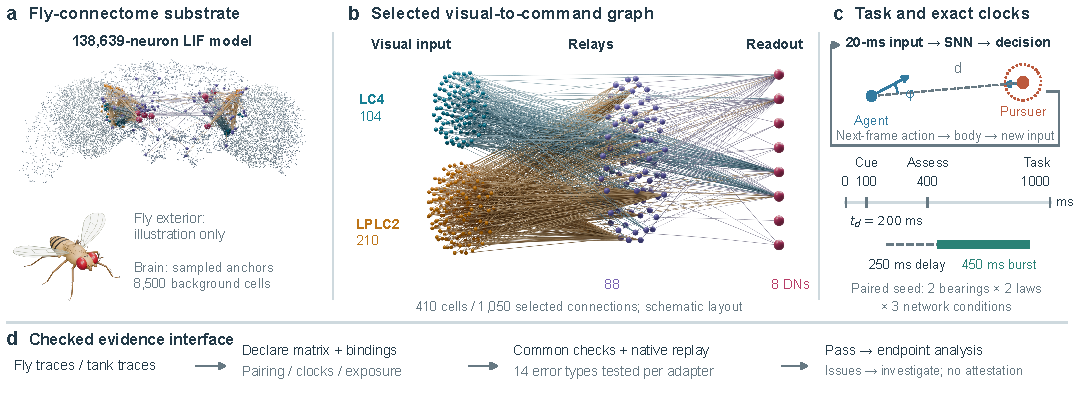
\includegraphics[width=\textwidth]{figs/evidence_v10_overview.pdf}
\caption{System and checked assessment interface. (a,b) Representative model anchors, an illustrative fly and a selected 410-cell/1,050-connection graph. The layout is schematic, not measured neurites or the complete recurrent graph. (c) Sampled feedback and exact burst events; $t_d=200$\,ms is illustrative. (d) Native traces enter common checks and independent replay before endpoint analysis.}
\label{fig:v10f-system}
\end{figure*}}
\newcommand{\ReuseCaption}{Cross-plant reuse and predefined error challenges. (a) First registered tank seed, high inflow, proportional law; level axis is zoomed, safe interval $[0.2,0.8]$. All 96 example tasks remain safe. (b) A requested outflow first changes at 0.60\,s and applies at 0.75\,s, between 100-ms frame boundaries. (c) Eleven common-checker and three native-only cases are detected per adapter, not a general coverage estimate.}
\newcommand{\WarningCaption}{Frozen secondary warning operating points. Rows state contact/success denominators; RF-0/A/B contain 24/12/12 independent seed clusters. Markers show missed-contact and false-alarm rates with pointwise 95\% whole-seed bootstrap CIs. Activity is two-sided; the forecast holds the current command using exact simulated state. Positive-class support is 12/2/1 seed clusters. Zero-width and class-conditional empirical intervals do not establish zero population risk.}
\iffourfigures
\newcommand{\reuseRef}{Fig.~\ref{fig:v10f-reuse}}
\newcommand{\warningRef}{Fig.~\ref{fig:v10f-warning}}
\newcommand{\ReuseFigure}{%
\begin{figure}[t]\centering
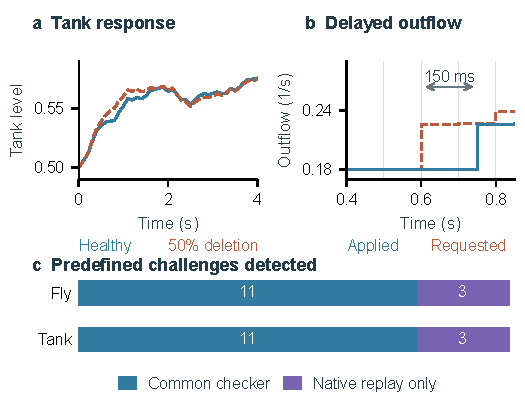
\includegraphics[width=\columnwidth]{figs/v10f_reuse.pdf}
\caption{\ReuseCaption}\label{fig:v10f-reuse}
\end{figure}}
\newcommand{\WarningFigure}{%
\begin{figure}[t]\centering
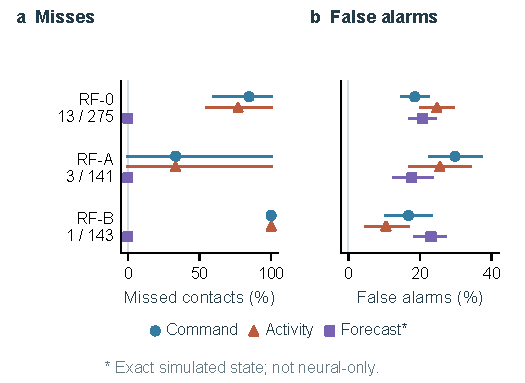
\includegraphics[width=\columnwidth]{figs/v10f_warning.pdf}
\caption{\WarningCaption}\label{fig:v10f-warning}
\end{figure}}
\else
\newcommand{\reuseRef}{Fig.~\ref{fig:v10f-reuse} (left)}
\newcommand{\warningRef}{Fig.~\ref{fig:v10f-warning} (right)}
\newcommand{\ReuseFigure}{%
\begin{figure*}[t]\centering
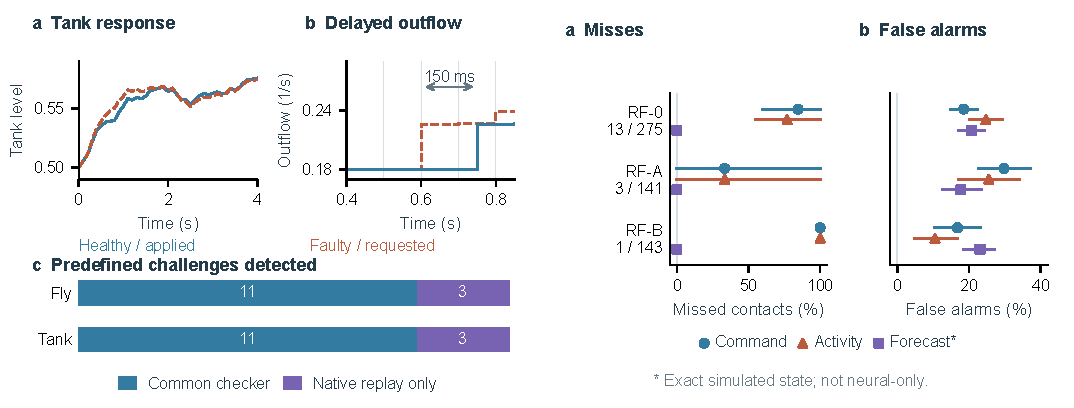
\includegraphics[width=\textwidth]{figs/v10f_reuse_warning.pdf}
\caption{\emph{Left:} \ReuseCaption\ \emph{Right:} \WarningCaption}
\label{fig:v10f-reuse}\label{fig:v10f-warning}
\end{figure*}}
\newcommand{\WarningFigure}{}
\fi
\newcommand{\TransferFigure}{%
\begin{figure*}[t]\centering
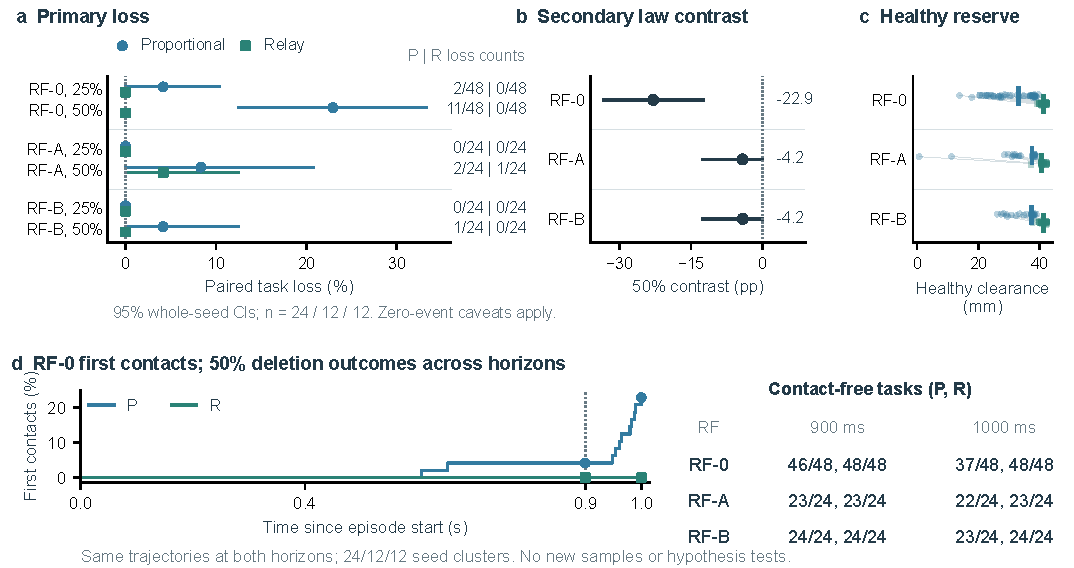
\includegraphics[width=\textwidth]{figs/v10h_rf.pdf}
\caption{Paired loss across sensory realizations and horizons. (a,b) Primary losses and prespecified secondary R-minus-P contrasts (percentage points), with pointwise 95\% whole-seed CIs, $n=24/12/12$, conditional on saved calibrations. All healthy tasks succeed; no gains occur. (c) Healthy minimum clearance shows unequal reserve. (d) RF-0/50\% first contacts and all-map 900/1000-ms success counts (P, R); both endpoints reuse the same 24/12/12 seed clusters, not new replicates or tests. Maps differ in draws, recalibration and cohorts, not an isolated RF effect.}
\label{fig:v10f-transfer}
\end{figure*}}

\section{Introduction and Positioning}
How do matched connection losses in a connectome-derived spiking neural network (SNN) affect collision outcomes as feedback, observation horizon and calibrated sensing change? Healthy binary success and early neural activity describe different aspects of this question. A task-level assessment must retain the pairing between damaged and healthy runs and identify when first contact occurs.

Shiu et al.\cite{shiu2024drosophila} establish connectome-derived LIF sensorimotor predictions; here the output drives a synthetic pursuit--escape plant. An\cite{an2026sparse} studies task- and state-dependent preservation under sparsification, and Jo\cite{jo2026simulating} couples damaged circuits to virtual-arena behavior. Our comparison instead targets paired geometric first contact under two frozen feedback laws and a declared horizon. Our warning target is subsequent contact from a 400-ms prefix, rather than identification of a damaged network. These are distinct evaluation questions, not claims that task dependence or neural/behavioral dissociation is new.

DriveFI searches faults and scenarios that violate closed-loop driving safety\cite{jha2019drivefi}; SpikeFI, SpikingJET and enpheeph provide configurable SNN injection campaigns\cite{spyrou2024spikefi,gogebakan2024spikingjet,colucci2022enpheeph}. Common random numbers\cite{glasserman1992crn}, hybrid-trajectory monitoring\cite{donze2010breach}, task/resource benchmarking\cite{yik2023neurobench,dangelo2026embodied} and physical fault propagation\cite{chessa2026crosslayer} are established. Our evidence interface checks supplied paired records and native replay obligations, complementing injection and violation search.

We contribute three concrete findings and capabilities: (i) a paired first-contact characterization in which RF-0 proportional 50\%-deletion losses rise from 2/48 to 11/48 between 900 and 1000\,ms, with no relay contacts, alongside smaller uncertain contrasts in separately recalibrated RF cohorts; (ii) a frozen-prefix evaluation exposing 11/13 missed RF-0 contacts and cross-configuration false alarms, limiting substitution of the tested scalar warnings for task outcomes; and (iii) executable pairing, timing and exposure contracts, checked against archived actuator/endpoint errors and reused on a delayed tank. These distinguish declared schedules from realized actuation before task loss or activity exposure is interpreted.

\SystemFigure
\ReuseFigure
\TransferFigure
\section{Neural Experiment and Statistical Design}
\subsection{Network, Feedback and Calibration}
The FlyWire v783-derived model\cite{dorkenwald2024neuronal} has 138,639 LIF neurons and 15,091,983 signed, contact-weighted connection rows. We use Shiu parameters\cite{shiu2024drosophila} in Brian~2\cite{stimberg2019brian2}, with 0.1-ms steps, 2.2-ms sensory refractoriness and state/weight restoration before each episode. Assumed Gaussian RFs stimulate 104 LC4 and 210 LPLC2 cells at up to 150\,Hz; other external rates are zero. Eight descending cells provide control features.

Between events, $\dot v=(v_0-v+g)/(20\,\mathrm{ms})$ and $\dot g=-g/(5\,\mathrm{ms})$. Threshold $-45$\,mV resets $v$ to $v_0=-52$\,mV and $g$ to zero; both equations pause during refractoriness. Recurrent events add signed contact count times 0.275\,mV to $g$ after 1.8\,ms. External events add 68.75\,mV to voltage. These are functional model parameters, not measured device-fault characteristics.

Input begins at 100\,ms; sensing and feedback update every 20\,ms. Bearing is world-relative angle minus heading; looming is the change of $\arctan(0.05/d)$ at actual separation $d$. The pursuer starts 0.25\,m away at $\pm30^\circ$ and moves at 0.3\,m/s. Each motion segment aims it at the agent's segment-start position. Both positions advance linearly using the agent's starting heading; heading updates at segment end, capped at $\pm100^\circ$. A frame-end decision affects the next frame. The first trigger schedules a 0.35-m/s, heading-fixed burst 250\,ms later for 450\,ms; otherwise speed is 0.05\,m/s. Segments split at exact actuator events; first contact with radius 0.05\,m is solved within each segment. Failure latches, while traces continue to $H=1$\,s for resource accounting. Post-contact activity is counterfactual and excluded from warnings.

For each map, 20 passive development episodes (four seeds, five bearings from $-60^\circ$ to $60^\circ$) fit an affine steering score $z$. Standardized five-frame means of eight command rates over 200--400\,ms predict bearing/$60^\circ$, using ridge penalty 10 and an unpenalized intercept. The trigger threshold is half the tenth percentile of development episode mean command rates over 200--300\,ms, floored at 2.5\,Hz. Before the cue or below threshold, steering is zero. Otherwise proportional/relay laws apply $-600\operatorname{clip}(z,-1,1)$/$-600\operatorname{sgn}(z)$ deg/s outside the burst. Healthy held-out validation RMSE is $65.9^\circ/67.8^\circ/67.2^\circ$ for RF-0/A/B, over eight seed clusters each: $z$ is not an accurate closed-loop bearing estimate.

\subsection{Pairing, Cohorts and Endpoints}
Shared uniforms give nested deletions $w_j^{(f)}=w_j\mathbf1[V_{sj}\geq f]$ and input events $\mathbf1[U_{sk\tau i}<\lambda_{ki}\Delta t]$. Indices denote seed $s$, frame $k$, neural step $\tau$, cell $i$ and connection row $j$; $\Delta t=10^{-4}$\,s. Feedback changes $\lambda$, while input variates and row masks remain paired. Seeds and hashes are traceable, without cross-platform bit-identity guarantees.

RF-0 uses 24 test seed clusters; RF-A/B each use 12 new clusters. Every cluster contains both bearings, two laws and healthy/25\%/50\% deletion: 288/144/144 episodes. New maps independently redraw all 314 azimuths from the same hemisphere prior (left $10$--$90^\circ$, right $-90$--$-10^\circ$), preserving identities, vertical mapping and gradients. Each separately fits the frozen development recipe, uses 32 healthy validation episodes in eight further clusters, then freezes thresholds before testing. All maps, seeds and failures are retained; no test tuning or efficacy stopping occurs. This is transfer with recalibration, not zero-shot transfer or an RF-isolated causal experiment.

With $Y=1$ meaning no contact through $H$, registered primary endpoints are paired loss $L=Y_H(1-Y_F)$, gain $G=(1-Y_H)Y_F$ and activity exposure. Net loss $D=L-G$ is derived. The relay-minus-proportional contrast and warnings are prespecified secondary; clearance/heading diagnostics are post-hoc. For cumulative spikes $S$ and $T_*=\min(T_F,T_H)$, own-stop and common-duration ratios are
\begin{equation}
R_{\rm stop}=\frac{S_F(T_F)}{S_H(T_H)},\qquad
R_{\rm common}=\frac{S_F(T_*)}{S_H(T_*)}.
\end{equation}
Here $T$ is contact-frame end or $H$, at 20-ms resolution. Common duration remains outcome-dependent and does not equate sensory histories; fixed 400-ms/1-s windows are separate endpoints.

Estimates average both bearings within seed. Pointwise 95\% CIs use 20,000 whole-seed percentile resamples, conditional on stored map/calibration/thresholds (RNG 20261022 for RF-0; 20261023 for transfer). Symmetric-null sign-flip sensitivity tests are Holm-adjusted over two baseline doses, separately from four new map/dose contrasts. Maps and separate angle/action cohorts are not pooled.

Warnings use only data through 400\,ms: unsmoothed 20-ms command rates averaged over 100--400\,ms, or the absolute log spike-count ratio to a law/bearing-specific healthy reference. Each RF's healthy validation separately sets fifth-percentile command/forecast and 95th-percentile two-sided activity cutoffs, frozen before its test cohort; an upper-only comparator flags activity above twice its healthy reference. A held-command forecast uses exact simulated geometry and pending actuation, retaining the current turn; its schedule-only baseline sets future turn to zero. These information-rich forecasts are not neural-only detectors.

\section{Executable Evidence Contract}
A campaign declares seed, condition, law, fault, horizon $H$, frame duration and resource unit. Adapters normalize native traces into those identities, source/map/calibration bindings, input/mask digests, completed observations, cumulative resource and first failure. Hashes bind bytes, not execution. Common checks test matrix membership, pairing, clocks, exposure, resources and outcome labels; native replay separately regenerates inputs and plant transitions. Shared variates need not produce identical feedback-dependent events. Warning prefixes exclude future labels.

Native timing checks require burst onset 250\,ms after the trigger, 450\,ms duration, and an active-at-$H$ flag consistent with that interval. In 72 separate historical records, an audit found 17 delays of 260\,ms, four completed bursts of 440\,ms and six incorrect horizon flags. These overlapping categories are not pooled with current cohorts. Ignoring them would misstate fast-motion duration or actuation at the endpoint. Replay therefore checks realized events, rather than accepting nominal parameters. Core-schema findings retain row indices; arbitrary native semantics remain adapter obligations.

\reuseRef\ adapts the same checker to a delayed tank: $\dot h=I-u-0.04h$, $h(0)=0.5$, safe interval $[0.2,0.8]$. Eight seeds, two inflows, two laws and three sensor-deletion levels (0/25/50\%) give 96 examples. Deleted samples hold their last value. Independent analytic replay checks sensor accounting and 150-ms delayed actuation on a 100-ms grid. All examples remain safe: they demonstrate reuse, not neural fault tolerance.

The original challenge set detects eleven common-checker and three native-only cases per adapter, not general coverage. A synthetic zero-neural-readout logger passes input/plant replay without solving neural equations: consistent traces cannot authenticate execution, unlogged state or safety.

\section{Results and Conditional Interpretation}
\subsection{First-Contact Loss Depends on the Declared Horizon}
Both laws completed 48/48 healthy RF-0 tasks. Fig.~\ref{fig:v10f-transfer}d gives 900/1000-ms success counts for all three RFs at 50\% deletion. RF-0 has nine additional P contacts in the final 100\,ms, the latest at 999.962\,ms; the law-discordant RF-A/B contacts also occur after 900\,ms. These are same-trajectory descriptive rescorings, not new samples or confirmatory horizon tests. RF-0's registration already lists these repeated endpoints. Conditional task preservation means no first contact through the stated endpoint.

At the registered 1-s endpoint, the prespecified secondary R-minus-P net-loss contrast was $-22.9$\,pp (95\% CI $[-33.3,-12.5]$; Holm $p=0.00195$). RF-A/B each yielded $-4.2$\,pp, CI $[-12.5,0]$; all four new map/dose Holm $p$ values are 1. Each new 50\% contrast has only one nonzero cluster. The smaller point estimates neither establish equivalence nor identify a causal RF effect; no between-map effect-change test is claimed. The baseline 25\% contrast remains uncertain ($p=0.50$). No 25\% loss occurs in A/B; twelve event-free clusters still allow a one-sided 95\% upper bound of 22.1\% for any loss in a new identically defined two-bearing cluster.

RF-0 healthy P/R median clearance was 33.1/41.4\,mm, with absolute heading at 400\,ms of $88.3^\circ/100^\circ$. Unequal reserve and the accumulation of late contacts are possible contributors to the observed law contrast, not isolated mechanisms. Separate RF calibrations and test cohorts also change together. RF-A's three 50\% contacts include both laws at seed 3009/$+30^\circ$ and P at 3011/$-30^\circ$; RF-B has P contact at 3110/$-30^\circ$. The law-discordant transfer contacts occur near 995\,ms. Healthy success, finite-horizon preservation and intrinsic damage tolerance are therefore different claims.

\subsection{Frozen Scalar Warnings Miss Subsequent Contacts}
\WarningFigure
The tested operating points ask whether fixed scalar prefixes suffice to flag later first contact, not whether an optimal neural predictor exists. Across healthy/25\%/50\% conditions, the command warning detected 2/13 RF-0 contacts, 2/3 in A and 0/1 in B (\warningRef); successful-task false alarms were 51/275, 42/141 and 24/143. The upper-only activity rule detected none. Exact-state held-command forecasts detected all observed contacts but falsely flagged 57/275, 25/141 and 33/143 successes; baseline schedule-only false alarms were 84/275. Their access to geometry and pending actuation precludes a neural-only detector comparison.

RF-0/A/B sensitivities have only 12/2/1 failure clusters. Of 20,000 resamples, 2,217/7,099 lack a positive class in A/B; those draws are omitted only for the corresponding conditional rate. Zero-width empirical intervals do not establish zero population risk. Own-stop/common-duration medians coincide in these campaigns (maximum paired difference below 0.006), so the historical large exposure artifact does not recur. P/50\% median 400-ms/1-s activity ratios remain 0.981/1.505, 0.961/1.212 and 0.956/1.139. A separate eight-cluster $\pm45^\circ$ test flags 22/32 healthy activity records and retains an uncertain law contrast. These results bound the tested frozen criteria, not all neural monitoring.

\section{Scope, Artifacts and Conclusion}
The evidence concerns one graph, an assumed RF family, a synthetic plant, unequal healthy reserve and sparse failures. The roughly $66^\circ$ held-out steering error is not accurate bearing reconstruction. Walk-only contact by 0.8\,s follows from plant speeds, not connectome advantage. Functional row loss establishes no biological tolerance, device upset rate, hardware safety, energy or area benefit; record consistency does not authenticate neural execution.

The generating snapshot\cite{artifactV10} preserves original sources, 576 neural records, 96 tank examples and frozen configurations. The fixed assessment revision\cite{artifactV10Horizon} provides schema guards, horizon-analysis sources and file manifests. Saved-record analysis/replay needs no external matrices; fresh neural runs require separately obtained, hash-matched inputs. Third-party tables with unresolved redistribution terms are excluded. Generation metadata remain unchanged.

The measured knowledge is conditional: matched deletion yields different first-contact timing under two feedback laws, the 1-s contrast is smaller and uncertain in recalibrated RF cohorts, and the tested frozen scalar prefixes retain task-label errors. Healthy clearance and horizon sensitivity delimit, rather than explain away, these observations. The checked interface makes the supporting pairs and clocks testable across two plant schemas. This task-level assessment provides a basis for evaluating how future device-level nonidealities propagate through neuromorphic controllers to closed-loop behavior.

\FloatBarrier\clearpage
\bibliographystyle{IEEEtran}
\bibliography{refs}
\end{document}
